\section*{Приборы и принадлежности}

Установка для исследования эффекта Холла включает:

\begin{itemize}
	\item датчик Холла \textbf{ДХ}, выполненный в виде пленки, напыленной на подложку из диэлектрика с четырьмя электродами для подведения электрического тока и измерения разности потенциалов Холла;
	\item электромагнит \textbf{ЭМ-} состоящий из соосной системы двух круговых катушек с током, расположенных на
	сердечнике из магнитомягкого материала;
	\item источников питания $ E_1 $ и $ E_2 $;
	\item потенциометр $ R_1 $ «\textbf{Ток ДХ}»,регулирующий ток $ I_1 $ через \textbf{ДХ};
	\item потенциометр $ R_2 $ «\textbf{Ток ЭМ}», регулирующий ток $ I_2 $ через электромагнит \textbf{ЭМ};
	\item миллиамперметр \textbf{mA}, измеряющий ток $ I_1 $ через \textbf{ДХ};
	\item вольтметр \textbf{V}$_2$, измеряющий падение напряжения на резисторе $ R $. Поскольку сопротивление $ R = 1 $ Ом ---
	значение напряжения $ U_2 $ численно равно $ I_2 $;
	\item операционный усилитель \textbf{ОУ} с коэффициентом усиления $ k $;
	\item вольтметр \textbf{V}$_1$, измеряющий напряжение $ U_1 $ на выходе \textbf{ОУ}, пропорциональное ЭДС на выходе датчика Холла
	$ U_x $. 

\end{itemize}

\newpage

Установка представлена на рис. \ref{schema}

\begin{figure}[hpt!]
	\centering
	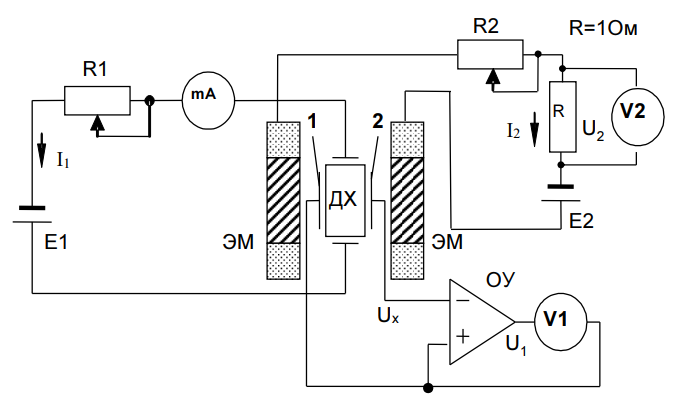
\includegraphics[width=0.8\linewidth]{photo/schema}
	\caption{Схема установки для исследования эффекта Холла}
	\label{schema}
\end{figure}

